\documentclass[11pt]{beamer}
\mode<presentation>
\let\Tiny=\tiny
\usetheme{CambridgeUS}
\usefonttheme{professionalfonts}
\usepackage[brazil]{babel}
\usepackage[utf8]{inputenc}

\title{Personas e Cenários}
\author{}}
\date{}

\begin{document}

   \begin{frame}[plain]
        \titlepage
   \end{frame}

   \section{Introdução}

   \begin{frame}{Introdução}
      \begin{itemize}
         \item Algumas experiências bem sucedidas, como Facebook, criaram o mito que para se ter sucesso basta ter inspiração.
         \item \textit{Softwares} construídos somente com base na inspiração tendem fracassar miseravelmente.
         \item A inspiração, nestes casos, não atende às reais necessidades do usuário.
         \item E mesmo em casos onde \textit{softwares} feitos "apenas" com inspiração são bem sucedidos, é necessário entender como ele é utilizado e quais suas lacunas.
      \end{itemize}
   \end{frame}

   \begin{frame}{Introdução}
      Em termos materiais, há três fatores comuns que impulsionam a criação de produtos de \textit{software}:
      \begin{itemize}
         \item necessidades de negócio e de consumo não atendidas pelos produtos atuais;
         \item insatisfação com os produtos de \textit{software} atuais;
         \item mudanças na tecnologia.
       \end{itemize}
   \end{frame}

   \begin{frame}{Introdução}
      \begin{itemize}
         \item Diferentemente dos projetos de software, os produtos de \textit{software} não são resultado dos requisitos de um cliente específico, mas é interessante conhecer seus usuários e clientes potenciais.
         \item Há diversas técnicas formais para estudo desses usuários, algumas caras e até mesmo infactíveis.
         \item Outra abordagem é utilizar maneiras mais informais, porém que podem trazer grande valor às etapas iniciais de desenvolvimento do produto de \textit{software}.
         \item O objetivo é, a partir do conhecimento sobre estes usuários, elaborar funcionalidades e restrições.
      \end{itemize}
   \end{frame}

   \begin{frame}{Funcionalidades e restrições}
      \begin{itemize}
         \item Funcionalidades são o que o usuário pode fazer no \textit{software}.
         \item Na literatura as funcionalidades também recebem o nome de requisitos funcionais.
         \item O usuário postar uma foto é um exemplo de funcionalidade.
      \end{itemize}
   \end{frame}

   \begin{frame}{Funcionalidades e restrições}
      \begin{itemize}
         \item Restrições são limitações impostas sobre o \textit{software}.
         \item Na literatura também são conhecidas como requisitos não-funcionais.
         \item O \textit{software} ter de rodar nos sistemas operacionais Linux, Windows e MacOS é um exemplo de restrição.
      \end{itemize}
   \end{frame}

   \section{Personas}

   \begin{frame}{Personas}
      \begin{itemize}
         \item Como dito anteriormente, o primeiro ponto é saber quem vai usar o produto de \textit{software}.
         \item Muitas vezes conhece-se alguma pessoa que possui o perfil de usuário, porém nem todos da equipe de desenvolvimento podem ter essa mesma noção.
         \item Por isso, é interessante a criação de personas.
      \end{itemize}
   \end{frame}

   \begin{frame}{Personas}
      "Persona é uma representação dos usuários mais comuns, baseada em uma parcela de tarefas críticas." (Tomlin, 2018; tradução nossa)
   \end{frame}

   \begin{frame}{Personas}
      \begin{itemize}
         \item Personas são "usuários imaginários", como personagens de um livro de ficção inspirados em pessoas reais.
         \item A persona é utilizada para mapear as necessidades e como as pessoas utilizam a aplicação no seu dia-a-dia.
         \item Por exemplo, se você está desenvolvendo um \textit{software} para escritórios de advocacia, um advogado, um recepcionista, um assistente legal são bons exemplos de personas a serem criados.
      \end{itemize}
   \end{frame}

   \begin{frame}{Personas}
      Há quatro razões principais para o uso de personas:
      \begin{itemize}
         \item adicionar contexto aos dados de UX comportamental;
         \item permitir o projeto centrado no usuário;
         \item ajudar no recrutamento para teste de usabilidade;
         \item diminuir o *scope creep*.
      \end{itemize}
   \end{frame}

   \begin{frame}{Personas}
      \begin{itemize}
         \item Com o uso de personas, pode-se analisar os dados de UX comportamental para definir não apenas como cada persona utiliza a aplicação, mas qual a relevância desta persona no uso da aplicação.
      \end{itemize}   
   \end{frame}

   \begin{frame}{Personas}
      \begin{itemize}
         \item Tenha-se um caso onde dois projetos de \textit{interface} completamente diferentes estão em disputa. 
         \item A partir disto, pode-se escolher o projeto de \textit{interface} baseado em resultados mais sólidos.
         \item O uso de personas contextualiza e agrupa usuários, facilitando aos tomadores de decisão verem o que fazer.
      \end{itemize}
   \end{frame}

   \begin{frame}{Personas}
      \begin{itemize}
         \item As personas também servem para delinear o escopo do projeto.
         \item Elas servem para lembrar a todos os envolvidos quais são os pontos mais importantes.
         \item Não apenas reduz o chamado \textit{scope creep}\footnote{quando o escopo cresce demasiadamente com o desenvolvimento do projeto}, mas permite traçar o caminho para a construção de um produto viável mínimo (MVP).
      \end{itemize}
   \end{frame}

   \begin{frame}
      Tomlin coloca alguns pontos importantes a serem levados em conta para criação de personas:
      \begin{itemize}
         \item são baseadas em pesquisas de campo;
         \item identificam padrões comuns de comportamento;
         \item focam no agora e não no futuro potencial das coisas;
         \item incluem foto, nome e estória breve;
         \item descrevem um problema ou tarefa que uma pessoa está tentando resolver;
         \item boas personas incluem ambientes típicos e/ou dispositivos utilizados;
         \item incluem a familiaridade da pessoa com o domínio do problema;
         \item definem duas ou três tarefas principais que a persona precisa realizar.
      \end{itemize}
   \end{frame}

   \begin{frame}{Personas}
      Tomlin coloca como atributos comuns de uma persona\footnote{Par}:
      \begin{itemize}
         \item foto;
         \item tarefas críticas;
         \item cenário e \textit{background};
         \item dispositivos;
         \item \textit{expertise} do domínio;
         \item ambiente;         
       \end{itemize}
   \end{frame}

   \begin{frame}{Personas}
      \begin{figure}
         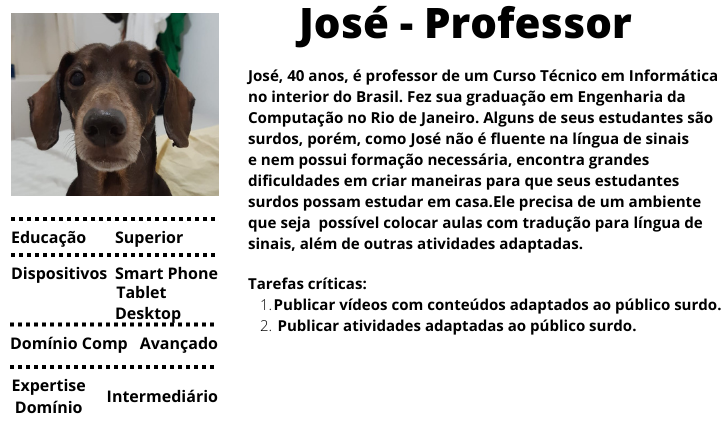
\includegraphics[width=10cm, height=6cm]{figures/persona.png}
      \end{figure}   
   \end{frame}

   \begin{frame}{Personas}
      \begin{itemize}
         \item Para criação de personas, Tomlin dá bastan\te ênfase à aquisição de informações.
         \item Ele sistematiza a investigação contextual de conduta.
      \end{itemize}
   \end{frame}

   \begin{frame}{Investigação contextual de conduta}
      "Investigação contextual de conduta é um método de pesquisa etnográfica para projeto centrado no usuário em que o pesquisador encontra os usuário no local e observa como eles interagem com sistemas no seu próprio ambiente." (Tomlin, 2018; tradução nossa)
   \end{frame}

   \begin{frame}{Investigação contextual de conduta}
      São etapas da investigação contextual de conduta:
      \begin{enumerate}
         \item preparação;
         \item encontrar as pessoas a serem observadas;
         \item sessão de observação;
         \item consolidação e análise dos dados coletados.
      \end{enumerate}
   \end{frame}

   \begin{frame}{Investigação contextual de conduta - preparação}
      A preparação envolve decidir:
      \begin{itemize}
         \item quem será observado;
         \item onde será observado;
         \item o que será observado;
         \item quais perguntas serão feitas.
      \end{itemize}
   \end{frame}

   \begin{frame}{Investigação contextual de conduta - encontrar pessoas}
      \begin{itemize}
         \item Para encontrar pessoas a serem observadas, em alguns casos, basta ir às ruas.
         \item Em outros casos, como juizes, empresários, médicos e outros profissionais que não estão comumente em público, mas em ambientes fechados, é necessário um esforço adicional.
         \item Pode-se utilizar contatos próprios e/ou recrutadores.
      \end{itemize}
   \end{frame}

   \begin{frame}{Investigação contextual de conduta - encontrar pessoas}
      Para convencer as pessoas a participar do estudo, deve-se evitar palavras como:
      \begin{itemize}
         \item pesquisa;
         \item observação;
         \item teste;
         \item estudo;
      \end{itemize}
      No lugar, deve-se dizer que busca-se "conhecer um pouco mais" o que a pessoa faz.
   \end{frame}

   \begin{frame}{Investigação contextual de conduta - encontrar pessoas}
      \begin{itemize}
         \item Deve-se ter muito cuidado com a privacidade e a anonimicidade do estudo.
         \item As pessoas que confiam que o que for dito ou observado durante o estudo não será compartilhado tendem a expor mais suas ideias.
      \end{itemize}
   \end{frame}

   \begin{frame}{Investigação contextual de conduta - sessão de observação}
      Tomlin sugere que a equipe de pesquisa siga alguns pontos:
      \begin{itemize}
         \item ser sempre cordial com os observados;
         \item calma ao ouvir/observar;
         \item prestar atenção até mesmo em expressões não verbais;
         \item perguntar o porquê das respostas ou ações;
         \item anotar ao máximo.
      \end{itemize}
   \end{frame}

   \begin{frame}{Investigação contextual de conduta - consolidação dos dados}
      \begin{itemize}
         \item a consolidação dos dados deve ser feita de maneira imediata para que não se percam detalhes.
         \item quanto mais distante a consolidação e análise de dados é feita, mais chances da equipe de pesquisa esquecer pontos que podem ser muito importantes.
      \end{itemize}
   \end{frame}

   \section{Cenários}

   \begin{frame}{Cenários}
      \begin{itemize}
         \item Sommerville recomenda o uso de cenários para descobrir as funcionalidades.
         \item O cenário é a narrativa que descreve uma dada situação em que um usuário (uma persona) está interagindo com o \textit{software}.
         \item Deve descrever o problema do usuário e como ele fará para resolvê-lo.
         \item Não é necessário descrever o sistema nos mínimos detalhes.
      \end{itemize}
   \end{frame}

   \begin{frame}{Cenários}
      Um cenário deve conter:
      \begin{itemize}
         \item uma breve afirmação sobre seu objetivo geral;
         \item referências à persona envolvida e suas motivações;
         \item informação sobre o que está envolvido na atividade;
         \item se apropriado, explicação dos problemas que não poderão ser resolvidos com o sistema e de como estes problemas poderão ser resolvidos.
      \end{itemize}
   \end{frame}

   \begin{frame}{Cenários}
      "José está ensinando o básico de \textit{hardware} para a turma e nela está um estudante surdo. José leva a turma para o laboratório de manutenção e demonstra as peças, uma a uma, com ajuda do intérprete de língua de sinais. Entretanto, o estudante surdo tem dificuldade em assimilar os novos sinais para as peças. Por isso, José precisa que o estudante tenha material para estudar em casa e fixar os novos termos.\\
      Então, José, com auxílio do intérprete, cria um vídeo mostrando as peças do computador e seus nomes em português e em LIBRAS. José autentica-se no Portal Mão Amiga e vai à tela de criar aula. Preenche os dados da aula e sobe o vídeo, além de outros materiais didáticos de apoio."
   \end{frame}

   \begin{frame}{Cenários}
      \begin{itemize}
         \item A escrita de um cenário deve começar a partir de uma ou mais personas criadas.
         \item Os cenários surgem a partir da imaginação sobre o que esta persona pode realizar com o \textit{software}.
         \item A escrita de cenários não possui uma fórmula exata e vai depender do produto de software e seus objetivos.
         \item Alguns cenários falarão mais de mecanismos e outros menos. Porém, o objetivo é que sejam claros o bastante para que até uma pessoa leiga entenda.
         \item Não são necessários cenários para todos os possíveis usos do software. Eles devem servir como auxílio e não como um ponto de lentidão.
      \end{itemize}
   \end{frame}

   \begin{frame}{Referências}
      \begin{itemize}
         \item Tomlin, W. Craig. UX Optimization: Combining Behavioral UX and Usability Testing Data to Optimize Websites. 1ed. 2018. APress.
         \item Sommerville, Ian. Engineering Software Products: An Introduction to Modern Software Engineering. 1ed. 2021. Pearson Education.
      \end{itemize}
   \end{frame}  
\end{document}